\documentclass[tikz,border=8pt]{standalone}
\usetikzlibrary{positioning,decorations.pathreplacing,arrows.meta}
\begin{document}
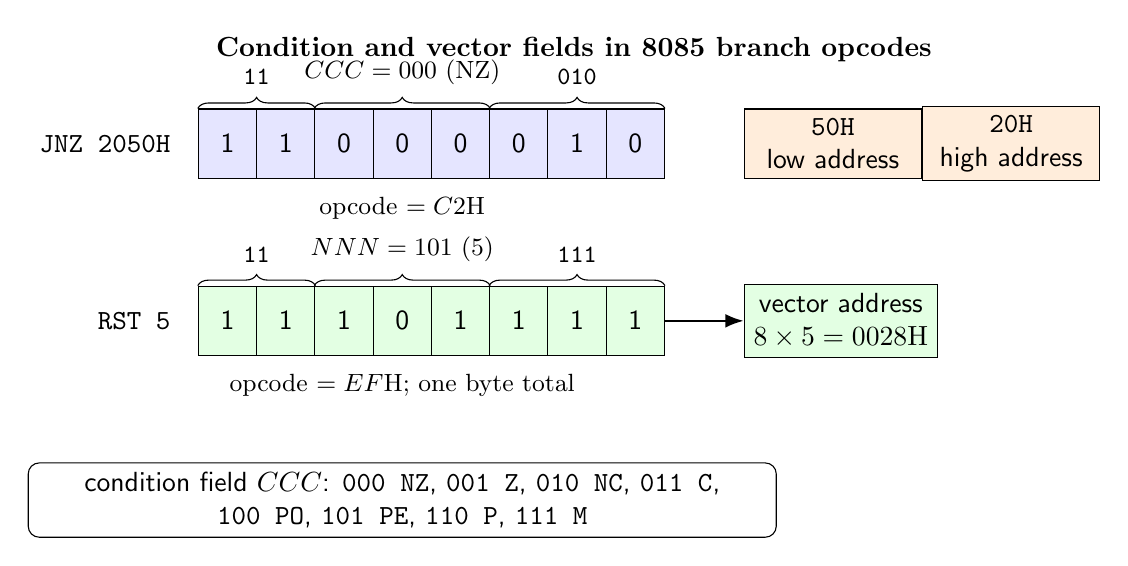
\begin{tikzpicture}[
  font=\sffamily,
  >=Latex,
  bit/.style={draw,minimum width=0.74cm,minimum height=0.88cm},
  byte/.style={draw,minimum width=2.25cm,minimum height=0.88cm,align=center},
  flow/.style={->,thick}
]
\node[font=\bfseries] at (5.0,4.0) {Condition and vector fields in 8085 branch opcodes};

\node[anchor=east,font=\bfseries] at (0,2.8) {\texttt{JNZ 2050H}};
\foreach \b [count=\i from 0] in {1,1,0,0,0,0,1,0}{
  \node[bit,fill=blue!10] (j\i) at (0.6+0.74*\i,2.8) {\b};
}
\draw[decorate,decoration={brace,amplitude=4pt}] (j0.north west)--(j1.north east)
 node[midway,above=5pt,font=\small]{\texttt{11}};
\draw[decorate,decoration={brace,amplitude=4pt}] (j2.north west)--(j4.north east)
 node[midway,above=5pt,font=\small]{$CCC=000$ (NZ)};
\draw[decorate,decoration={brace,amplitude=4pt}] (j5.north west)--(j7.north east)
 node[midway,above=5pt,font=\small]{\texttt{010}};
\node[byte,fill=orange!14,right=1.0cm of j7] (jlo) {\texttt{50H}\\low address};
\node[byte,fill=orange!14,right=0pt of jlo] (jhi) {\texttt{20H}\\high address};
\node[below=3pt of j3,font=\small] {opcode $=C2\mathrm{H}$};

\node[anchor=east,font=\bfseries] at (0,0.55) {\texttt{RST 5}};
\foreach \b [count=\i from 0] in {1,1,1,0,1,1,1,1}{
  \node[bit,fill=green!11] (r\i) at (0.6+0.74*\i,0.55) {\b};
}
\draw[decorate,decoration={brace,amplitude=4pt}] (r0.north west)--(r1.north east)
 node[midway,above=5pt,font=\small]{\texttt{11}};
\draw[decorate,decoration={brace,amplitude=4pt}] (r2.north west)--(r4.north east)
 node[midway,above=5pt,font=\small]{$NNN=101$ (5)};
\draw[decorate,decoration={brace,amplitude=4pt}] (r5.north west)--(r7.north east)
 node[midway,above=5pt,font=\small]{\texttt{111}};
\node[byte,fill=green!11,right=1.0cm of r7] (vec) {vector address\\$8\times5=0028\mathrm{H}$};
\draw[flow] (r7.east) -- (vec.west);
\node[below=3pt of r3,font=\small] {opcode $=EF\mathrm{H}$; one byte total};

\node[draw,rounded corners,below=1.35cm of r3,align=center,minimum width=9.5cm] (conds)
 {condition field $CCC$: \texttt{000 NZ}, \texttt{001 Z}, \texttt{010 NC}, \texttt{011 C},\\
  \texttt{100 PO}, \texttt{101 PE}, \texttt{110 P}, \texttt{111 M}};
\end{tikzpicture}
\end{document}
